\section{Aufbau}
\label{sec:Aufbau}
Der verwendete Aufbau ist in \autoref{fig:aufbau} dargestellt. Er besteht aus einer Rubidiumdampflampe, um Photonen
mit der Energie der $D_1$-Linie zu emittieren. Das Licht wird anschließen durch eine Linse gebündelt, mit Hilfe
Interferenzfilters auf die $D_1$-Komponente reduziert und durch ein $\lambda/4$-Plättchen zirkular polarisiert.
Danach durchquert es eine mit Rubidiumdampf gefüllte Zelle, um durch eine weiter Linse fokussiert zu werden und
an einer Photodiode detektiert zu werden. Die Rubidium Zelle wird auf $\SI{50}{\celsius}$ geheizt, um Dampf zu
erzeugen.
\begin{figure}
    \centering
    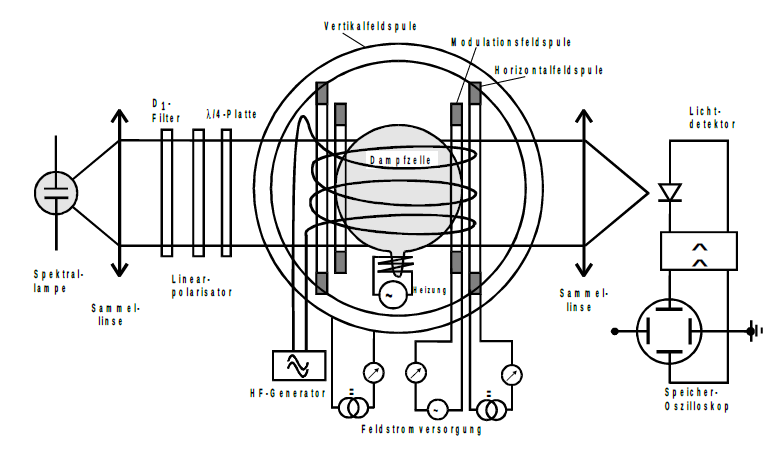
\includegraphics[scale=0.8]{aufbau.png}
    \caption{Schematische Darstellung des verwendeten Versuchaufbaus. \cite{V21}}
    \label{fig:aufbau}
\end{figure}
Die Zelle wird von drei Helmholtzspulenpaaren umgeben. Ein Vertikales, das dazu verwendet wird das Erdmagnetfeld
auszugleichen. Die anderen beiden werden in der Horizontalen verwendet, um das RF-Feld
zu erzeugen. Die Ausgabe der Photodiode kann an einem Oszilloskop abgelesen werden, das es im Sweep-Modus erlaubt
verschiedene Feldstärken zu überstreichen, um eine möglichst genaue Messung zu bekommen. Der Aufbau wird nach der
entsprechenden Justierung abgedeckt, um Umwelteinflüsse möglichst gering zu halten.

\section{Durchführung}
\label{sec:Durchführung}
Zu Beginn wird der Versuchsaufbau justiert und der Tisch in Richtung des Erdmagnetfelds ausgerichtet. Auf dem
Oszilloskop ist nach Einschalten der Apparatur ein breiter Peak zu sehen, der sich auf das Abfallen der
Transparenz bei fehlendem Magnetfeld zurück führen lässt. Durch Einstellen des Vertikalfeldes wird nun das
Erdmagnetfeld kompensiert und dadurch der Peak schmaller gemacht. Danach werden die beiden Rubidiumisotope auf
ihre Resonanzstellen untersucht. Dazu wird die RF-Spule eingeschaltet und Messwerte im Bereich von
$\SI{100}{\kilo\hertz}$ bis $\SI{1}{\mega\hertz}$ in $\SI{100}{\kilo\hertz}$-Schritten aufgenommen. Für die
höheren Frequenzen wird zusätzlich noch ein anderes horizontales Feld angelegt. Außerdem wird noch ein Bild eines
typischen Kurvenverlaufs am Oszilloskops fotografiert.